% Options for packages loaded elsewhere
\PassOptionsToPackage{unicode}{hyperref}
\PassOptionsToPackage{hyphens}{url}
\documentclass[
]{article}
\usepackage{xcolor}
\usepackage[margin=1in]{geometry}
\usepackage{amsmath,amssymb}
\setcounter{secnumdepth}{-\maxdimen} % remove section numbering
\usepackage{iftex}
\ifPDFTeX
  \usepackage[T1]{fontenc}
  \usepackage[utf8]{inputenc}
  \usepackage{textcomp} % provide euro and other symbols
\else % if luatex or xetex
  \usepackage{unicode-math} % this also loads fontspec
  \defaultfontfeatures{Scale=MatchLowercase}
  \defaultfontfeatures[\rmfamily]{Ligatures=TeX,Scale=1}
\fi
\usepackage{lmodern}
\ifPDFTeX\else
  % xetex/luatex font selection
\fi
% Use upquote if available, for straight quotes in verbatim environments
\IfFileExists{upquote.sty}{\usepackage{upquote}}{}
\IfFileExists{microtype.sty}{% use microtype if available
  \usepackage[]{microtype}
  \UseMicrotypeSet[protrusion]{basicmath} % disable protrusion for tt fonts
}{}
\makeatletter
\@ifundefined{KOMAClassName}{% if non-KOMA class
  \IfFileExists{parskip.sty}{%
    \usepackage{parskip}
  }{% else
    \setlength{\parindent}{0pt}
    \setlength{\parskip}{6pt plus 2pt minus 1pt}}
}{% if KOMA class
  \KOMAoptions{parskip=half}}
\makeatother
\usepackage{color}
\usepackage{fancyvrb}
\newcommand{\VerbBar}{|}
\newcommand{\VERB}{\Verb[commandchars=\\\{\}]}
\DefineVerbatimEnvironment{Highlighting}{Verbatim}{commandchars=\\\{\}}
% Add ',fontsize=\small' for more characters per line
\usepackage{framed}
\definecolor{shadecolor}{RGB}{248,248,248}
\newenvironment{Shaded}{\begin{snugshade}}{\end{snugshade}}
\newcommand{\AlertTok}[1]{\textcolor[rgb]{0.94,0.16,0.16}{#1}}
\newcommand{\AnnotationTok}[1]{\textcolor[rgb]{0.56,0.35,0.01}{\textbf{\textit{#1}}}}
\newcommand{\AttributeTok}[1]{\textcolor[rgb]{0.13,0.29,0.53}{#1}}
\newcommand{\BaseNTok}[1]{\textcolor[rgb]{0.00,0.00,0.81}{#1}}
\newcommand{\BuiltInTok}[1]{#1}
\newcommand{\CharTok}[1]{\textcolor[rgb]{0.31,0.60,0.02}{#1}}
\newcommand{\CommentTok}[1]{\textcolor[rgb]{0.56,0.35,0.01}{\textit{#1}}}
\newcommand{\CommentVarTok}[1]{\textcolor[rgb]{0.56,0.35,0.01}{\textbf{\textit{#1}}}}
\newcommand{\ConstantTok}[1]{\textcolor[rgb]{0.56,0.35,0.01}{#1}}
\newcommand{\ControlFlowTok}[1]{\textcolor[rgb]{0.13,0.29,0.53}{\textbf{#1}}}
\newcommand{\DataTypeTok}[1]{\textcolor[rgb]{0.13,0.29,0.53}{#1}}
\newcommand{\DecValTok}[1]{\textcolor[rgb]{0.00,0.00,0.81}{#1}}
\newcommand{\DocumentationTok}[1]{\textcolor[rgb]{0.56,0.35,0.01}{\textbf{\textit{#1}}}}
\newcommand{\ErrorTok}[1]{\textcolor[rgb]{0.64,0.00,0.00}{\textbf{#1}}}
\newcommand{\ExtensionTok}[1]{#1}
\newcommand{\FloatTok}[1]{\textcolor[rgb]{0.00,0.00,0.81}{#1}}
\newcommand{\FunctionTok}[1]{\textcolor[rgb]{0.13,0.29,0.53}{\textbf{#1}}}
\newcommand{\ImportTok}[1]{#1}
\newcommand{\InformationTok}[1]{\textcolor[rgb]{0.56,0.35,0.01}{\textbf{\textit{#1}}}}
\newcommand{\KeywordTok}[1]{\textcolor[rgb]{0.13,0.29,0.53}{\textbf{#1}}}
\newcommand{\NormalTok}[1]{#1}
\newcommand{\OperatorTok}[1]{\textcolor[rgb]{0.81,0.36,0.00}{\textbf{#1}}}
\newcommand{\OtherTok}[1]{\textcolor[rgb]{0.56,0.35,0.01}{#1}}
\newcommand{\PreprocessorTok}[1]{\textcolor[rgb]{0.56,0.35,0.01}{\textit{#1}}}
\newcommand{\RegionMarkerTok}[1]{#1}
\newcommand{\SpecialCharTok}[1]{\textcolor[rgb]{0.81,0.36,0.00}{\textbf{#1}}}
\newcommand{\SpecialStringTok}[1]{\textcolor[rgb]{0.31,0.60,0.02}{#1}}
\newcommand{\StringTok}[1]{\textcolor[rgb]{0.31,0.60,0.02}{#1}}
\newcommand{\VariableTok}[1]{\textcolor[rgb]{0.00,0.00,0.00}{#1}}
\newcommand{\VerbatimStringTok}[1]{\textcolor[rgb]{0.31,0.60,0.02}{#1}}
\newcommand{\WarningTok}[1]{\textcolor[rgb]{0.56,0.35,0.01}{\textbf{\textit{#1}}}}
\usepackage{graphicx}
\makeatletter
\newsavebox\pandoc@box
\newcommand*\pandocbounded[1]{% scales image to fit in text height/width
  \sbox\pandoc@box{#1}%
  \Gscale@div\@tempa{\textheight}{\dimexpr\ht\pandoc@box+\dp\pandoc@box\relax}%
  \Gscale@div\@tempb{\linewidth}{\wd\pandoc@box}%
  \ifdim\@tempb\p@<\@tempa\p@\let\@tempa\@tempb\fi% select the smaller of both
  \ifdim\@tempa\p@<\p@\scalebox{\@tempa}{\usebox\pandoc@box}%
  \else\usebox{\pandoc@box}%
  \fi%
}
% Set default figure placement to htbp
\def\fps@figure{htbp}
\makeatother
\setlength{\emergencystretch}{3em} % prevent overfull lines
\providecommand{\tightlist}{%
  \setlength{\itemsep}{0pt}\setlength{\parskip}{0pt}}
\usepackage{fontspec}
\setmainfont{Times New Roman}  % Replace with a Unicode-friendly font installed on your system
\usepackage{bookmark}
\IfFileExists{xurl.sty}{\usepackage{xurl}}{} % add URL line breaks if available
\urlstyle{same}
\hypersetup{
  pdftitle={Imports ARIMA},
  pdfauthor={Andrew Jowe},
  hidelinks,
  pdfcreator={LaTeX via pandoc}}

\title{Imports ARIMA}
\author{Andrew Jowe}
\date{}

\begin{document}
\maketitle

\section{Col Removal}\label{col-removal}

Keep Year, Imports, and GDP columns

\begin{Shaded}
\begin{Highlighting}[]
\NormalTok{finalPro\_data }\OtherTok{\textless{}{-}}\NormalTok{ finalPro\_data[, }\FunctionTok{c}\NormalTok{(}\StringTok{"Year"}\NormalTok{, }\StringTok{"Imports"}\NormalTok{)]}
\end{Highlighting}
\end{Shaded}

\section{Plot Time Series}\label{plot-time-series}

\begin{Shaded}
\begin{Highlighting}[]
\CommentTok{\# Plot Imports}
\NormalTok{imports\_ts }\OtherTok{\textless{}{-}} \FunctionTok{ts}\NormalTok{(finalPro\_data}\SpecialCharTok{$}\NormalTok{Imports, }\AttributeTok{start =} \DecValTok{1960}\NormalTok{, }\AttributeTok{frequency =} \DecValTok{1}\NormalTok{)}

\FunctionTok{ts.plot}\NormalTok{(imports\_ts, }\AttributeTok{main=}\StringTok{"Imports Time Series"}\NormalTok{, }\AttributeTok{ylab=}\StringTok{"Imports"}\NormalTok{)}
\end{Highlighting}
\end{Shaded}

\pandocbounded{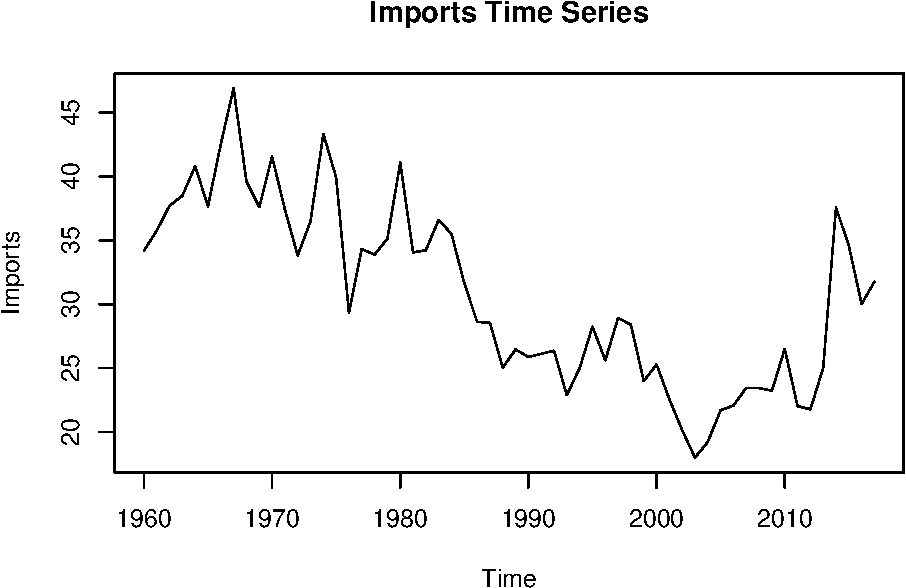
\includegraphics[keepaspectratio]{final_imports_files/figure-latex/unnamed-chunk-3-1.pdf}}

Summary: - Imports time series has upward trend, this shows this is
non-stationary - It has peaks around every 10 year: 1980, 1990, 2010

\section{Transform}\label{transform}

\begin{Shaded}
\begin{Highlighting}[]
\CommentTok{\# Box{-}Cox transform Imports}
\NormalTok{lambda }\OtherTok{\textless{}{-}} \FunctionTok{BoxCox.lambda}\NormalTok{(imports\_ts)}
\NormalTok{boxcox\_imports\_ts }\OtherTok{\textless{}{-}}\NormalTok{ imports\_ts }\CommentTok{\# BoxCox(imports\_ts, lambda)}
\FunctionTok{ts.plot}\NormalTok{(boxcox\_imports\_ts, }\AttributeTok{main =} \FunctionTok{paste}\NormalTok{(}\StringTok{"Box{-}Cox Transformed Imports (lambda ="}\NormalTok{, }\FunctionTok{round}\NormalTok{(lambda, }\DecValTok{3}\NormalTok{), }\StringTok{")"}\NormalTok{), }\AttributeTok{ylab =} \StringTok{"Transformed Imports"}\NormalTok{)}
\end{Highlighting}
\end{Shaded}

\pandocbounded{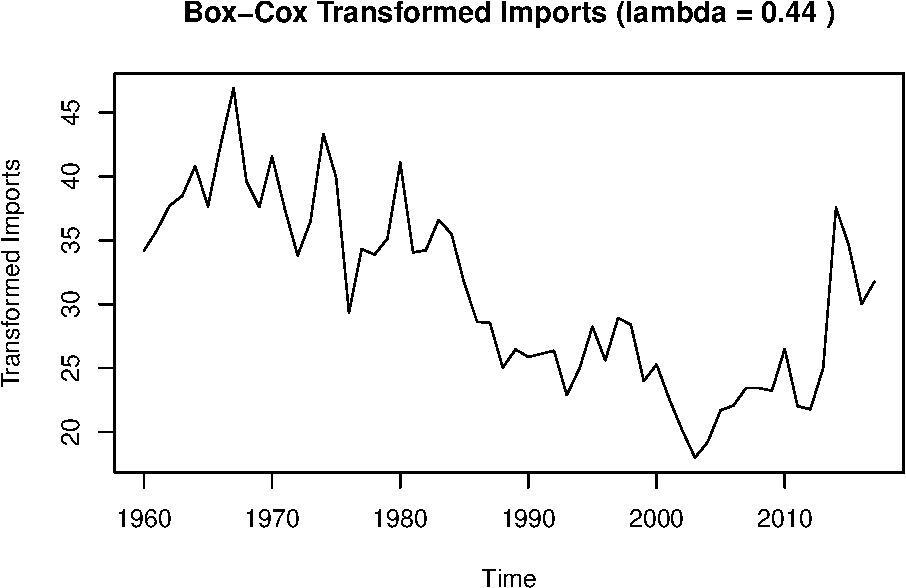
\includegraphics[keepaspectratio]{final_imports_files/figure-latex/unnamed-chunk-4-1.pdf}}

We tried log, but residuals not normal.

\section{Differencing Imports}\label{differencing-imports}

\begin{Shaded}
\begin{Highlighting}[]
\NormalTok{diff\_imports\_bc }\OtherTok{\textless{}{-}} \FunctionTok{diff}\NormalTok{(boxcox\_imports\_ts, }\AttributeTok{differences=}\DecValTok{1}\NormalTok{)}

\CommentTok{\# Plot differenced Box{-}Cox Imports}
\FunctionTok{ts.plot}\NormalTok{(diff\_imports\_bc, }\AttributeTok{main=}\StringTok{"Differenced Box{-}Cox Transformed Imports Time Series"}\NormalTok{, }\AttributeTok{ylab=}\StringTok{"Transformed Imports"}\NormalTok{)}
\end{Highlighting}
\end{Shaded}

\pandocbounded{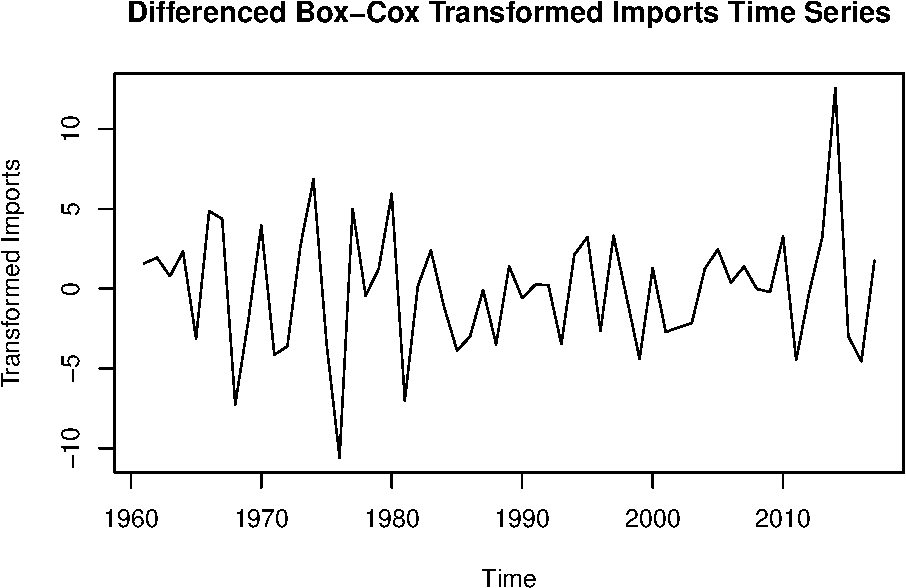
\includegraphics[keepaspectratio]{final_imports_files/figure-latex/unnamed-chunk-5-1.pdf}}

\section{Root test for stationarity
check}\label{root-test-for-stationarity-check}

\begin{Shaded}
\begin{Highlighting}[]
\CommentTok{\# Load tseries for ADF test}
\FunctionTok{library}\NormalTok{(tseries)}

\CommentTok{\# Augmented Dickey{-}Fuller Test}
\NormalTok{adf\_result }\OtherTok{\textless{}{-}} \FunctionTok{adf.test}\NormalTok{(diff\_imports\_bc)}
\end{Highlighting}
\end{Shaded}

\begin{verbatim}
## Warning in adf.test(diff_imports_bc): p-value smaller than printed p-value
\end{verbatim}

\begin{Shaded}
\begin{Highlighting}[]
\FunctionTok{cat}\NormalTok{(}\StringTok{"ADF test p{-}value:"}\NormalTok{, }\FunctionTok{round}\NormalTok{(adf\_result}\SpecialCharTok{$}\NormalTok{p.value, }\DecValTok{4}\NormalTok{), }
    \FunctionTok{ifelse}\NormalTok{(adf\_result}\SpecialCharTok{$}\NormalTok{p.value }\SpecialCharTok{\textless{}} \FloatTok{0.05}\NormalTok{, }\StringTok{"(PASS {-} Stationary)"}\NormalTok{, }\StringTok{"(FAIL {-} Non{-}stationary)"}\NormalTok{), }\StringTok{"}\SpecialCharTok{\textbackslash{}n}\StringTok{"}\NormalTok{)}
\end{Highlighting}
\end{Shaded}

\begin{verbatim}
## ADF test p-value: 0.01 (PASS - Stationary)
\end{verbatim}

\section{ACF / PACF plots}\label{acf-pacf-plots}

\begin{Shaded}
\begin{Highlighting}[]
\CommentTok{\# ACF and PACF of the transformed and differenced series}
\FunctionTok{par}\NormalTok{(}\AttributeTok{mfrow =} \FunctionTok{c}\NormalTok{(}\DecValTok{1}\NormalTok{, }\DecValTok{2}\NormalTok{))}
\FunctionTok{Acf}\NormalTok{(diff\_imports\_bc, }\AttributeTok{main =} \StringTok{"ACF of Imports"}\NormalTok{)}
\FunctionTok{Pacf}\NormalTok{(diff\_imports\_bc, }\AttributeTok{main =} \StringTok{"PACF of Imports"}\NormalTok{)}
\end{Highlighting}
\end{Shaded}

\pandocbounded{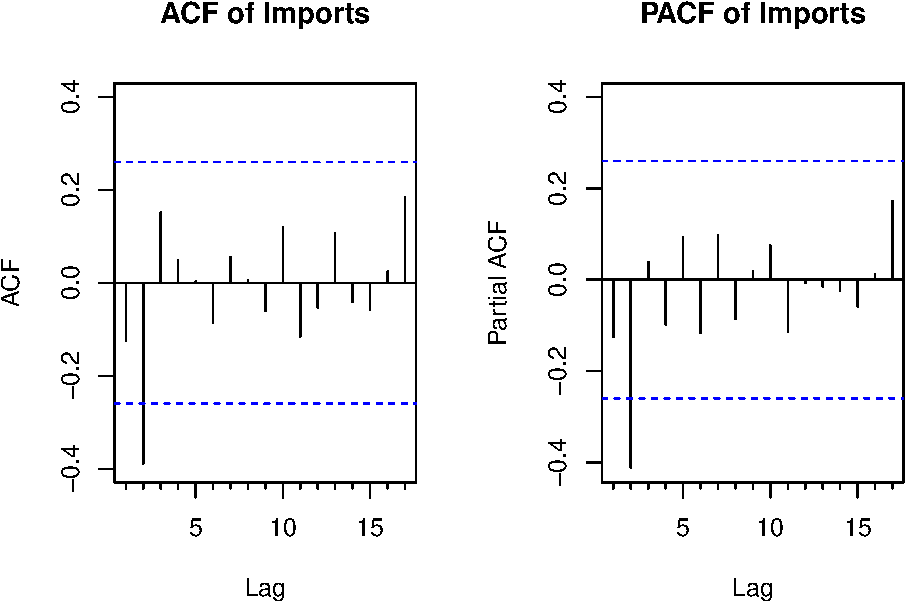
\includegraphics[keepaspectratio]{final_imports_files/figure-latex/unnamed-chunk-7-1.pdf}}

\begin{Shaded}
\begin{Highlighting}[]
\FunctionTok{par}\NormalTok{(}\AttributeTok{mfrow =} \FunctionTok{c}\NormalTok{(}\DecValTok{1}\NormalTok{, }\DecValTok{1}\NormalTok{))}
\end{Highlighting}
\end{Shaded}

\section{Modeling}\label{modeling}

\begin{Shaded}
\begin{Highlighting}[]
\CommentTok{\# Central African Republic Imports ARIMA Model}

\CommentTok{\# Diagnostics on chosen model}
\NormalTok{final\_model }\OtherTok{\textless{}{-}} \FunctionTok{Arima}\NormalTok{(boxcox\_imports\_ts, }\AttributeTok{order =} \FunctionTok{c}\NormalTok{(}\DecValTok{2}\NormalTok{, }\DecValTok{1}\NormalTok{, }\DecValTok{2}\NormalTok{), }\AttributeTok{method =} \StringTok{"ML"}\NormalTok{)}
\FunctionTok{print}\NormalTok{(final\_model)}
\end{Highlighting}
\end{Shaded}

\begin{verbatim}
## Series: boxcox_imports_ts 
## ARIMA(2,1,2) 
## 
## Coefficients:
##           ar1      ar2     ma1      ma2
##       -0.4076  -0.1258  0.2827  -0.3737
## s.e.   0.2738   0.2779  0.2598   0.2725
## 
## sigma^2 = 12.32:  log likelihood = -150.65
## AIC=311.3   AICc=312.48   BIC=321.51
\end{verbatim}

\begin{Shaded}
\begin{Highlighting}[]
\NormalTok{residuals\_final }\OtherTok{\textless{}{-}} \FunctionTok{residuals}\NormalTok{(final\_model)}

\CommentTok{\# Residual ACF and PACF for final model}
\FunctionTok{par}\NormalTok{(}\AttributeTok{mfrow =} \FunctionTok{c}\NormalTok{(}\DecValTok{1}\NormalTok{, }\DecValTok{2}\NormalTok{))  }\CommentTok{\# Side{-}by{-}side layout}
\FunctionTok{acf}\NormalTok{(residuals\_final, }\AttributeTok{main =} \StringTok{"ACF of Final Model Residuals"}\NormalTok{)}
\FunctionTok{pacf}\NormalTok{(residuals\_final, }\AttributeTok{main =} \StringTok{"PACF of Final Model Residuals"}\NormalTok{)}
\end{Highlighting}
\end{Shaded}

\pandocbounded{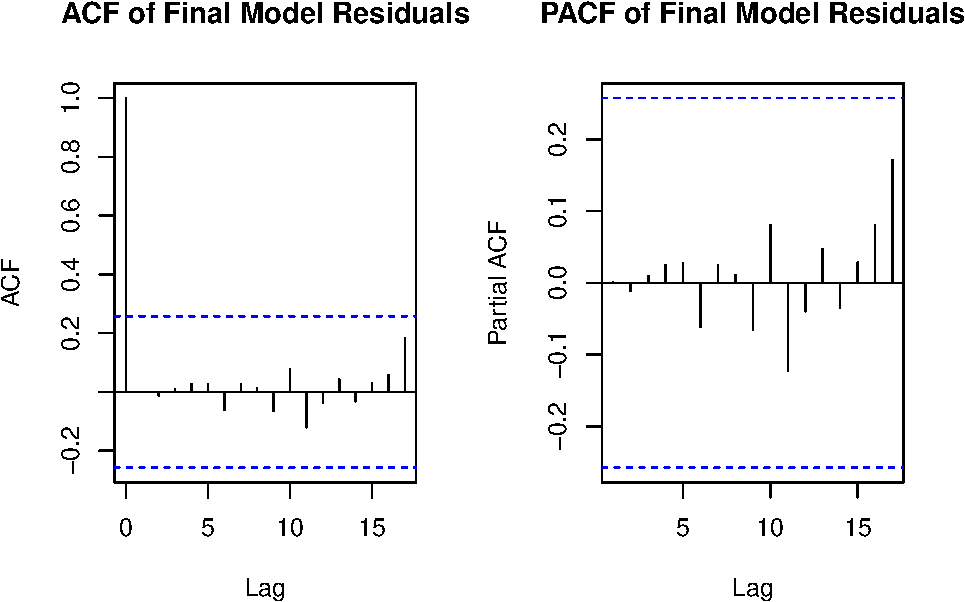
\includegraphics[keepaspectratio]{final_imports_files/figure-latex/unnamed-chunk-8-1.pdf}}

\begin{Shaded}
\begin{Highlighting}[]
\FunctionTok{par}\NormalTok{(}\AttributeTok{mfrow =} \FunctionTok{c}\NormalTok{(}\DecValTok{1}\NormalTok{, }\DecValTok{1}\NormalTok{))  }\CommentTok{\# Reset layout}

\CommentTok{\# Diagnostic Tests (Simplified)}
\FunctionTok{cat}\NormalTok{(}\StringTok{"}\SpecialCharTok{\textbackslash{}n}\StringTok{Diagnostic Tests (Simplified):}\SpecialCharTok{\textbackslash{}n}\StringTok{"}\NormalTok{)}
\end{Highlighting}
\end{Shaded}

\begin{verbatim}
## 
## Diagnostic Tests (Simplified):
\end{verbatim}

\begin{Shaded}
\begin{Highlighting}[]
\CommentTok{\# 1. Portmanteau (Ljung{-}Box) Test for Autocorrelation}
\NormalTok{ljung }\OtherTok{\textless{}{-}} \FunctionTok{Box.test}\NormalTok{(residuals\_final, }\AttributeTok{lag =} \DecValTok{10}\NormalTok{, }\AttributeTok{type =} \StringTok{"Ljung{-}Box"}\NormalTok{)}
\FunctionTok{cat}\NormalTok{(}\StringTok{"Ljung{-}Box test p{-}value:"}\NormalTok{, }\FunctionTok{round}\NormalTok{(ljung}\SpecialCharTok{$}\NormalTok{p.value, }\DecValTok{4}\NormalTok{), }
    \FunctionTok{ifelse}\NormalTok{(ljung}\SpecialCharTok{$}\NormalTok{p.value }\SpecialCharTok{\textgreater{}} \FloatTok{0.05}\NormalTok{, }\StringTok{"(PASS {-} residuals ≈ white noise)"}\NormalTok{, }\StringTok{"(FAIL)"}\NormalTok{), }\StringTok{"}\SpecialCharTok{\textbackslash{}n}\StringTok{"}\NormalTok{)}
\end{Highlighting}
\end{Shaded}

\begin{verbatim}
## Ljung-Box test p-value: 0.9997 (PASS - residuals ≈ white noise)
\end{verbatim}

\begin{Shaded}
\begin{Highlighting}[]
\CommentTok{\# 2. Shapiro{-}Wilk Test for Normality}
\CommentTok{\# this does not violate model assumptions, but it violates confidence interval assumptions}
\NormalTok{shapiro }\OtherTok{\textless{}{-}} \FunctionTok{shapiro.test}\NormalTok{(residuals\_final)}
\FunctionTok{cat}\NormalTok{(}\StringTok{"Shapiro{-}Wilk test p{-}value:"}\NormalTok{, }\FunctionTok{round}\NormalTok{(shapiro}\SpecialCharTok{$}\NormalTok{p.value, }\DecValTok{4}\NormalTok{), }
    \FunctionTok{ifelse}\NormalTok{(shapiro}\SpecialCharTok{$}\NormalTok{p.value }\SpecialCharTok{\textgreater{}} \FloatTok{0.05}\NormalTok{, }\StringTok{"(PASS {-} approx. normal residuals)"}\NormalTok{, }\StringTok{"(FAIL)"}\NormalTok{), }\StringTok{"}\SpecialCharTok{\textbackslash{}n}\StringTok{"}\NormalTok{)}
\end{Highlighting}
\end{Shaded}

\begin{verbatim}
## Shapiro-Wilk test p-value: 0.0022 (FAIL)
\end{verbatim}

\begin{Shaded}
\begin{Highlighting}[]
\CommentTok{\# STEP 3: Model Comparison}
\CommentTok{\# Expanded grid search from ARIMA(0,1,0) to ARIMA(4,1,4)}
\NormalTok{models }\OtherTok{\textless{}{-}} \FunctionTok{list}\NormalTok{()}
\ControlFlowTok{for}\NormalTok{ (p }\ControlFlowTok{in} \DecValTok{0}\SpecialCharTok{:}\DecValTok{4}\NormalTok{) \{}
  \ControlFlowTok{for}\NormalTok{ (q }\ControlFlowTok{in} \DecValTok{0}\SpecialCharTok{:}\DecValTok{4}\NormalTok{) \{}
\NormalTok{    name }\OtherTok{\textless{}{-}} \FunctionTok{paste0}\NormalTok{(}\StringTok{"ARIMA("}\NormalTok{, p, }\StringTok{",1,"}\NormalTok{, q, }\StringTok{")"}\NormalTok{)}
\NormalTok{    models[[name]] }\OtherTok{\textless{}{-}} \FunctionTok{c}\NormalTok{(p, }\DecValTok{1}\NormalTok{, q)}
\NormalTok{  \}}
\NormalTok{\}}
\NormalTok{results }\OtherTok{\textless{}{-}} \FunctionTok{data.frame}\NormalTok{(}\AttributeTok{Model=}\FunctionTok{character}\NormalTok{(), }\AttributeTok{AIC=}\FunctionTok{numeric}\NormalTok{(), }\AttributeTok{BIC=}\FunctionTok{numeric}\NormalTok{(), }
                     \AttributeTok{Ljung\_Box\_p=}\FunctionTok{numeric}\NormalTok{(), }\AttributeTok{stringsAsFactors=}\ConstantTok{FALSE}\NormalTok{)}

\ControlFlowTok{for}\NormalTok{(i }\ControlFlowTok{in} \DecValTok{1}\SpecialCharTok{:}\FunctionTok{length}\NormalTok{(models)) \{}
\NormalTok{  fit }\OtherTok{\textless{}{-}} \FunctionTok{Arima}\NormalTok{(boxcox\_imports\_ts, }\AttributeTok{order =}\NormalTok{ models[[i]], }\AttributeTok{method =} \StringTok{"ML"}\NormalTok{)}
\NormalTok{  ljung\_p }\OtherTok{\textless{}{-}} \FunctionTok{Box.test}\NormalTok{(}\FunctionTok{residuals}\NormalTok{(fit), }\AttributeTok{lag =} \DecValTok{10}\NormalTok{, }\AttributeTok{type =} \StringTok{"Ljung{-}Box"}\NormalTok{)}\SpecialCharTok{$}\NormalTok{p.value}
\NormalTok{  results }\OtherTok{\textless{}{-}} \FunctionTok{rbind}\NormalTok{(results, }\FunctionTok{data.frame}\NormalTok{(}
    \AttributeTok{Model =} \FunctionTok{names}\NormalTok{(models)[i],}
    \AttributeTok{AIC =}\NormalTok{ fit}\SpecialCharTok{$}\NormalTok{aic,}
    \AttributeTok{BIC =} \FunctionTok{BIC}\NormalTok{(fit),}
    \AttributeTok{Ljung\_Box\_p =}\NormalTok{ ljung\_p}
\NormalTok{  ))}
\NormalTok{\}}
\FunctionTok{print}\NormalTok{(results)}
\end{Highlighting}
\end{Shaded}

\begin{verbatim}
##           Model      AIC      BIC Ljung_Box_p
## 1  ARIMA(0,1,0) 316.3143 318.3573   0.1755999
## 2  ARIMA(0,1,1) 315.3522 319.4383   0.6210100
## 3  ARIMA(0,1,2) 309.3683 315.4975   0.9363533
## 4  ARIMA(0,1,3) 309.2473 317.4195   0.9997589
## 5  ARIMA(0,1,4) 311.2467 321.4620   0.9997698
## 6  ARIMA(1,1,0) 317.4368 321.5229   0.2515772
## 7  ARIMA(1,1,1) 314.9475 321.0767   0.7413242
## 8  ARIMA(1,1,2) 309.4892 317.6614   0.9995161
## 9  ARIMA(1,1,3) 311.2468 321.4620   0.9997687
## 10 ARIMA(1,1,4) 313.2469 325.5052   0.9997686
## 11 ARIMA(2,1,0) 308.9097 315.0388   0.9779056
## 12 ARIMA(2,1,1) 310.8015 318.9737   0.9749142
## 13 ARIMA(2,1,2) 311.2997 321.5149   0.9996982
## 14 ARIMA(2,1,3) 313.2449 325.5032   0.9997572
## 15 ARIMA(2,1,4) 315.2144 329.5157   0.9996537
## 16 ARIMA(3,1,0) 310.8494 319.0216   0.9762303
## 17 ARIMA(3,1,1) 311.6273 321.8425   0.9988347
## 18 ARIMA(3,1,2) 313.2359 325.4942   0.9997612
## 19 ARIMA(3,1,3) 315.2106 329.5120   0.9997852
## 20 ARIMA(3,1,4) 315.1932 331.5376   0.9977253
## 21 ARIMA(4,1,0) 312.4420 322.6573   0.9857691
## 22 ARIMA(4,1,1) 313.0303 325.2886   0.9998808
## 23 ARIMA(4,1,2) 311.8824 326.1837   0.9999999
## 24 ARIMA(4,1,3) 313.7943 330.1387   1.0000000
## 25 ARIMA(4,1,4) 317.1901 335.5776   0.9976952
\end{verbatim}

\begin{Shaded}
\begin{Highlighting}[]
\CommentTok{\# If we inspect the BIC too, the one with min AIC is likely to also have the min BIC}
\FunctionTok{cat}\NormalTok{(}\StringTok{"}\SpecialCharTok{\textbackslash{}n}\StringTok{Best model by AIC:"}\NormalTok{, results}\SpecialCharTok{$}\NormalTok{Model[}\FunctionTok{which.min}\NormalTok{(results}\SpecialCharTok{$}\NormalTok{AIC)], }\StringTok{"}\SpecialCharTok{\textbackslash{}n}\StringTok{"}\NormalTok{)}
\end{Highlighting}
\end{Shaded}

\begin{verbatim}
## 
## Best model by AIC: ARIMA(2,1,0)
\end{verbatim}

\begin{Shaded}
\begin{Highlighting}[]
\CommentTok{\# STEP 4: Final Model and Diagnostics}
\NormalTok{final\_model }\OtherTok{\textless{}{-}} \FunctionTok{Arima}\NormalTok{(boxcox\_imports\_ts, }\AttributeTok{order =} \FunctionTok{c}\NormalTok{(}\DecValTok{2}\NormalTok{, }\DecValTok{1}\NormalTok{, }\DecValTok{0}\NormalTok{), }\AttributeTok{method =} \StringTok{"ML"}\NormalTok{)}
\FunctionTok{print}\NormalTok{(final\_model)}
\end{Highlighting}
\end{Shaded}

\begin{verbatim}
## Series: boxcox_imports_ts 
## ARIMA(2,1,0) 
## 
## Coefficients:
##           ar1      ar2
##       -0.1727  -0.4101
## s.e.   0.1203   0.1197
## 
## sigma^2 = 12.25:  log likelihood = -151.45
## AIC=308.91   AICc=309.36   BIC=315.04
\end{verbatim}

\begin{Shaded}
\begin{Highlighting}[]
\NormalTok{residuals\_final }\OtherTok{\textless{}{-}} \FunctionTok{residuals}\NormalTok{(final\_model)}

\CommentTok{\# Residual ACF and PACF for final model}
\FunctionTok{par}\NormalTok{(}\AttributeTok{mfrow =} \FunctionTok{c}\NormalTok{(}\DecValTok{1}\NormalTok{, }\DecValTok{2}\NormalTok{))  }\CommentTok{\# Side{-}by{-}side layout}
\FunctionTok{acf}\NormalTok{(residuals\_final, }\AttributeTok{main =} \StringTok{"ACF of Final Model Residuals"}\NormalTok{)}
\FunctionTok{pacf}\NormalTok{(residuals\_final, }\AttributeTok{main =} \StringTok{"PACF of Final Model Residuals"}\NormalTok{)}
\end{Highlighting}
\end{Shaded}

\pandocbounded{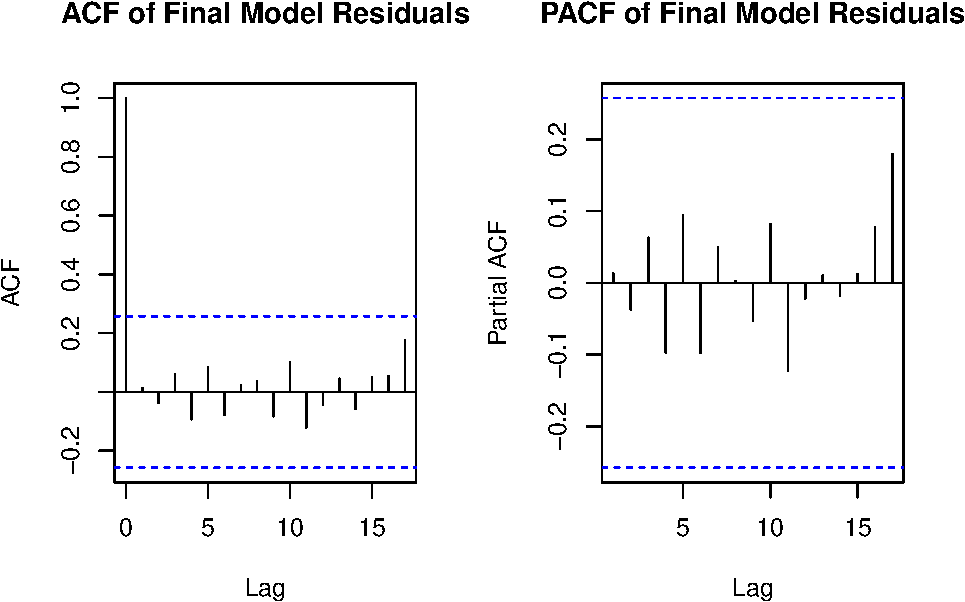
\includegraphics[keepaspectratio]{final_imports_files/figure-latex/unnamed-chunk-8-2.pdf}}

\begin{Shaded}
\begin{Highlighting}[]
\FunctionTok{par}\NormalTok{(}\AttributeTok{mfrow =} \FunctionTok{c}\NormalTok{(}\DecValTok{1}\NormalTok{, }\DecValTok{1}\NormalTok{))  }\CommentTok{\# Reset layout}

\FunctionTok{cat}\NormalTok{(}\StringTok{"}\SpecialCharTok{\textbackslash{}n}\StringTok{Diagnostic Tests:}\SpecialCharTok{\textbackslash{}n}\StringTok{"}\NormalTok{)}
\end{Highlighting}
\end{Shaded}

\begin{verbatim}
## 
## Diagnostic Tests:
\end{verbatim}

\begin{Shaded}
\begin{Highlighting}[]
\CommentTok{\# 1. Ljung{-}Box test}
\NormalTok{ljung }\OtherTok{\textless{}{-}} \FunctionTok{Box.test}\NormalTok{(residuals\_final, }\AttributeTok{lag =} \DecValTok{10}\NormalTok{, }\AttributeTok{type =} \StringTok{"Ljung{-}Box"}\NormalTok{)}
\FunctionTok{cat}\NormalTok{(}\StringTok{"Ljung{-}Box test p{-}value:"}\NormalTok{, }\FunctionTok{round}\NormalTok{(ljung}\SpecialCharTok{$}\NormalTok{p.value, }\DecValTok{4}\NormalTok{), }
    \FunctionTok{ifelse}\NormalTok{(ljung}\SpecialCharTok{$}\NormalTok{p.value }\SpecialCharTok{\textgreater{}} \FloatTok{0.05}\NormalTok{, }\StringTok{"(PASS)"}\NormalTok{, }\StringTok{"(FAIL)"}\NormalTok{), }\StringTok{"}\SpecialCharTok{\textbackslash{}n}\StringTok{"}\NormalTok{)}
\end{Highlighting}
\end{Shaded}

\begin{verbatim}
## Ljung-Box test p-value: 0.9779 (PASS)
\end{verbatim}

\begin{Shaded}
\begin{Highlighting}[]
\CommentTok{\# 2. Normality test}
\CommentTok{\# this does not violate model assumptions, but it violates confidence interval assumptions}
\NormalTok{shapiro }\OtherTok{\textless{}{-}} \FunctionTok{shapiro.test}\NormalTok{(residuals\_final)}
\FunctionTok{cat}\NormalTok{(}\StringTok{"Shapiro{-}Wilk test p{-}value:"}\NormalTok{, }\FunctionTok{round}\NormalTok{(shapiro}\SpecialCharTok{$}\NormalTok{p.value, }\DecValTok{4}\NormalTok{), }
    \FunctionTok{ifelse}\NormalTok{(shapiro}\SpecialCharTok{$}\NormalTok{p.value }\SpecialCharTok{\textgreater{}} \FloatTok{0.05}\NormalTok{, }\StringTok{"(PASS)"}\NormalTok{, }\StringTok{"(FAIL)"}\NormalTok{), }\StringTok{"}\SpecialCharTok{\textbackslash{}n}\StringTok{"}\NormalTok{)}
\end{Highlighting}
\end{Shaded}

\begin{verbatim}
## Shapiro-Wilk test p-value: 0.0253 (FAIL)
\end{verbatim}

\begin{Shaded}
\begin{Highlighting}[]
\CommentTok{\# 3. ARCH test}
\NormalTok{arch }\OtherTok{\textless{}{-}} \FunctionTok{Box.test}\NormalTok{(residuals\_final}\SpecialCharTok{\^{}}\DecValTok{2}\NormalTok{, }\AttributeTok{lag =} \DecValTok{5}\NormalTok{, }\AttributeTok{type =} \StringTok{"Ljung{-}Box"}\NormalTok{)}
\FunctionTok{cat}\NormalTok{(}\StringTok{"ARCH test p{-}value:"}\NormalTok{, }\FunctionTok{round}\NormalTok{(arch}\SpecialCharTok{$}\NormalTok{p.value, }\DecValTok{4}\NormalTok{), }
    \FunctionTok{ifelse}\NormalTok{(arch}\SpecialCharTok{$}\NormalTok{p.value }\SpecialCharTok{\textgreater{}} \FloatTok{0.05}\NormalTok{, }\StringTok{"(PASS)"}\NormalTok{, }\StringTok{"(FAIL)"}\NormalTok{), }\StringTok{"}\SpecialCharTok{\textbackslash{}n}\StringTok{"}\NormalTok{)}
\end{Highlighting}
\end{Shaded}

\begin{verbatim}
## ARCH test p-value: 0.9631 (PASS)
\end{verbatim}

\begin{Shaded}
\begin{Highlighting}[]
\FunctionTok{cat}\NormalTok{(}\StringTok{"}\SpecialCharTok{\textbackslash{}n}\StringTok{Slight non{-}normality detected but acceptable for ARIMA modeling}\SpecialCharTok{\textbackslash{}n}\StringTok{"}\NormalTok{)}
\end{Highlighting}
\end{Shaded}

\begin{verbatim}
## 
## Slight non-normality detected but acceptable for ARIMA modeling
\end{verbatim}

\begin{Shaded}
\begin{Highlighting}[]
\FunctionTok{cat}\NormalTok{(}\StringTok{"Q{-}Q plot shows approximate normality with minor tail deviations}\SpecialCharTok{\textbackslash{}n\textbackslash{}n}\StringTok{"}\NormalTok{)}
\end{Highlighting}
\end{Shaded}

\begin{verbatim}
## Q-Q plot shows approximate normality with minor tail deviations
\end{verbatim}

\begin{Shaded}
\begin{Highlighting}[]
\CommentTok{\# STEP 5: Forecast with Inverse Transformation}
\NormalTok{forecast\_result }\OtherTok{\textless{}{-}} \FunctionTok{forecast}\NormalTok{(final\_model, }\AttributeTok{h =} \DecValTok{3}\NormalTok{)}
\NormalTok{lambda }\OtherTok{\textless{}{-}} \FloatTok{0.1}
\CommentTok{\# Inverse Box{-}Cox transformation}
\NormalTok{forecast\_original }\OtherTok{\textless{}{-}}\NormalTok{ (lambda }\SpecialCharTok{*}\NormalTok{ forecast\_result}\SpecialCharTok{$}\NormalTok{mean }\SpecialCharTok{+} \DecValTok{1}\NormalTok{)}\SpecialCharTok{\^{}}\NormalTok{(}\DecValTok{1}\SpecialCharTok{/}\NormalTok{lambda)}
\NormalTok{lower\_original }\OtherTok{\textless{}{-}}\NormalTok{ (lambda }\SpecialCharTok{*}\NormalTok{ forecast\_result}\SpecialCharTok{$}\NormalTok{lower }\SpecialCharTok{+} \DecValTok{1}\NormalTok{)}\SpecialCharTok{\^{}}\NormalTok{(}\DecValTok{1}\SpecialCharTok{/}\NormalTok{lambda)}
\NormalTok{upper\_original }\OtherTok{\textless{}{-}}\NormalTok{ (lambda }\SpecialCharTok{*}\NormalTok{ forecast\_result}\SpecialCharTok{$}\NormalTok{upper }\SpecialCharTok{+} \DecValTok{1}\NormalTok{)}\SpecialCharTok{\^{}}\NormalTok{(}\DecValTok{1}\SpecialCharTok{/}\NormalTok{lambda)}
\FunctionTok{cat}\NormalTok{(}\StringTok{"1{-}step ahead forecast (original Imports scale):"}\NormalTok{, }\FunctionTok{round}\NormalTok{(forecast\_original[}\DecValTok{1}\NormalTok{], }\DecValTok{2}\NormalTok{), }\StringTok{"Imports}\SpecialCharTok{\textbackslash{}n}\StringTok{"}\NormalTok{)}
\end{Highlighting}
\end{Shaded}

\begin{verbatim}
## 1-step ahead forecast (original Imports scale): 2338369 Imports
\end{verbatim}

\begin{Shaded}
\begin{Highlighting}[]
\FunctionTok{cat}\NormalTok{(}\StringTok{"95\% prediction interval: ["}\NormalTok{, }\FunctionTok{round}\NormalTok{(lower\_original[}\DecValTok{1}\NormalTok{,}\DecValTok{2}\NormalTok{], }\DecValTok{2}\NormalTok{), }\StringTok{","}\NormalTok{, }
    \FunctionTok{round}\NormalTok{(upper\_original[}\DecValTok{1}\NormalTok{,}\DecValTok{2}\NormalTok{], }\DecValTok{2}\NormalTok{), }\StringTok{"] Imports}\SpecialCharTok{\textbackslash{}n\textbackslash{}n}\StringTok{"}\NormalTok{)}
\end{Highlighting}
\end{Shaded}

\begin{verbatim}
## 95% prediction interval: [ 417519 , 10162153 ] Imports
\end{verbatim}

\begin{Shaded}
\begin{Highlighting}[]
\FunctionTok{cat}\NormalTok{(}\StringTok{"FINAL MODEL: ARIMA(2, 1, 0) for Box{-}Cox transformed Imports}\SpecialCharTok{\textbackslash{}n}\StringTok{"}\NormalTok{)}
\end{Highlighting}
\end{Shaded}

\begin{verbatim}
## FINAL MODEL: ARIMA(2, 1, 0) for Box-Cox transformed Imports
\end{verbatim}

\section{Forecast next 10 periods using the best
model}\label{forecast-next-10-periods-using-the-best-model}

\begin{Shaded}
\begin{Highlighting}[]
\NormalTok{forecast\_horizon }\OtherTok{\textless{}{-}} \DecValTok{10}
\NormalTok{imports\_forecast }\OtherTok{\textless{}{-}} \FunctionTok{forecast}\NormalTok{(final\_model, }\AttributeTok{h =}\NormalTok{ forecast\_horizon)}

\CommentTok{\# Plot the forecast}
\FunctionTok{autoplot}\NormalTok{(imports\_forecast) }\SpecialCharTok{+}
  \FunctionTok{ggtitle}\NormalTok{(}\StringTok{"ARIMA Forecast of Imports (in Millions $)"}\NormalTok{) }\SpecialCharTok{+}
  \FunctionTok{xlab}\NormalTok{(}\StringTok{"Year"}\NormalTok{) }\SpecialCharTok{+}
  \FunctionTok{ylab}\NormalTok{(}\StringTok{"Imports"}\NormalTok{) }\SpecialCharTok{+}
  \FunctionTok{theme\_minimal}\NormalTok{()}
\end{Highlighting}
\end{Shaded}

\pandocbounded{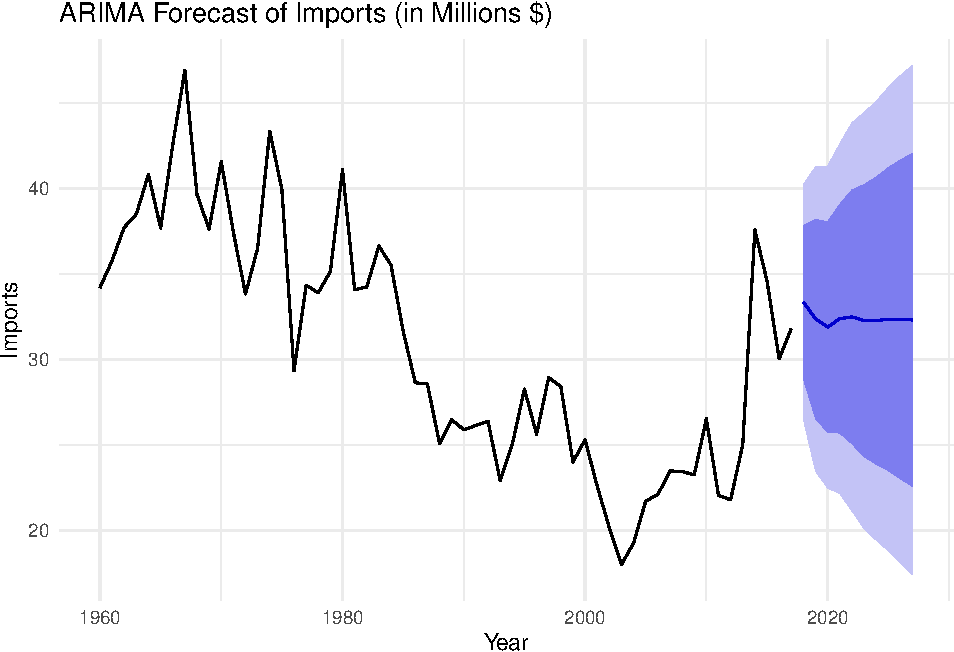
\includegraphics[keepaspectratio]{final_imports_files/figure-latex/unnamed-chunk-9-1.pdf}}

\end{document}
